\chapter{Аналитический раздел}
В данном разделе будет проанализирована поставленная задача, определён необходимый функционал програмного обеспечения, описаны роли пользователей программы и будет произведён анализ существующих моделей базы данных.

\section{Постановка задачи}
Необходимо разработать программу для отображения информации \newline интернет-магазина парфюмерии. Покупатель должен иметь возможность просмотра каталога товаров, оформления зазаза выбранной продукции, написания отзывов к товарам и постановки оценок товарам. Необходимо предусмотреть наличие ролей менеджера и администратора, осуществляющих управление продукцией, заказами и регулярующих деятельность покупателей.
\section{Формализация данных}

\captionsetup{singlelinecheck = false, justification=raggedright}
\begin{table}[h!]
	\begin{center}
		\caption{Данные и сведения о них}
		\begin{tabular}{ |p{5cm}|p{11cm}| }
			\hline
			\textbf{Данные} & \textbf{Сведения}\\ \hline
			Пользователь &  ФИО, никнейм, дата рождения, адрес, e-mail, пароль, права доступа, пол, аватар\\ \hline
			Товар &  Заголовок, описание, фото, категории,\ количество, стоимость, дата публикации, объем флакона, рейтинг\\ \hline
			Заказ &  Товары, дата оформления, дата исполнения,\ стоимость, статус, комментарий\\ \hline
			Отзыв &  Содержание, дата, пользователь, рейтинг, дата\ публикации\\ \hline
			Оценка &  Дата, значение, пользователь\\ \hline
		\end{tabular}
		\label{data-table}
	\end{center}
\end{table}		

\newpage

\section{ER-диаграмма сущностей}

На рисунке \ref{er_diagram} представлена ER-диаграмма сущностей проекта.

\captionsetup{singlelinecheck = false, justification=centering}
\begin{figure}[h!]
	\begin{center}
		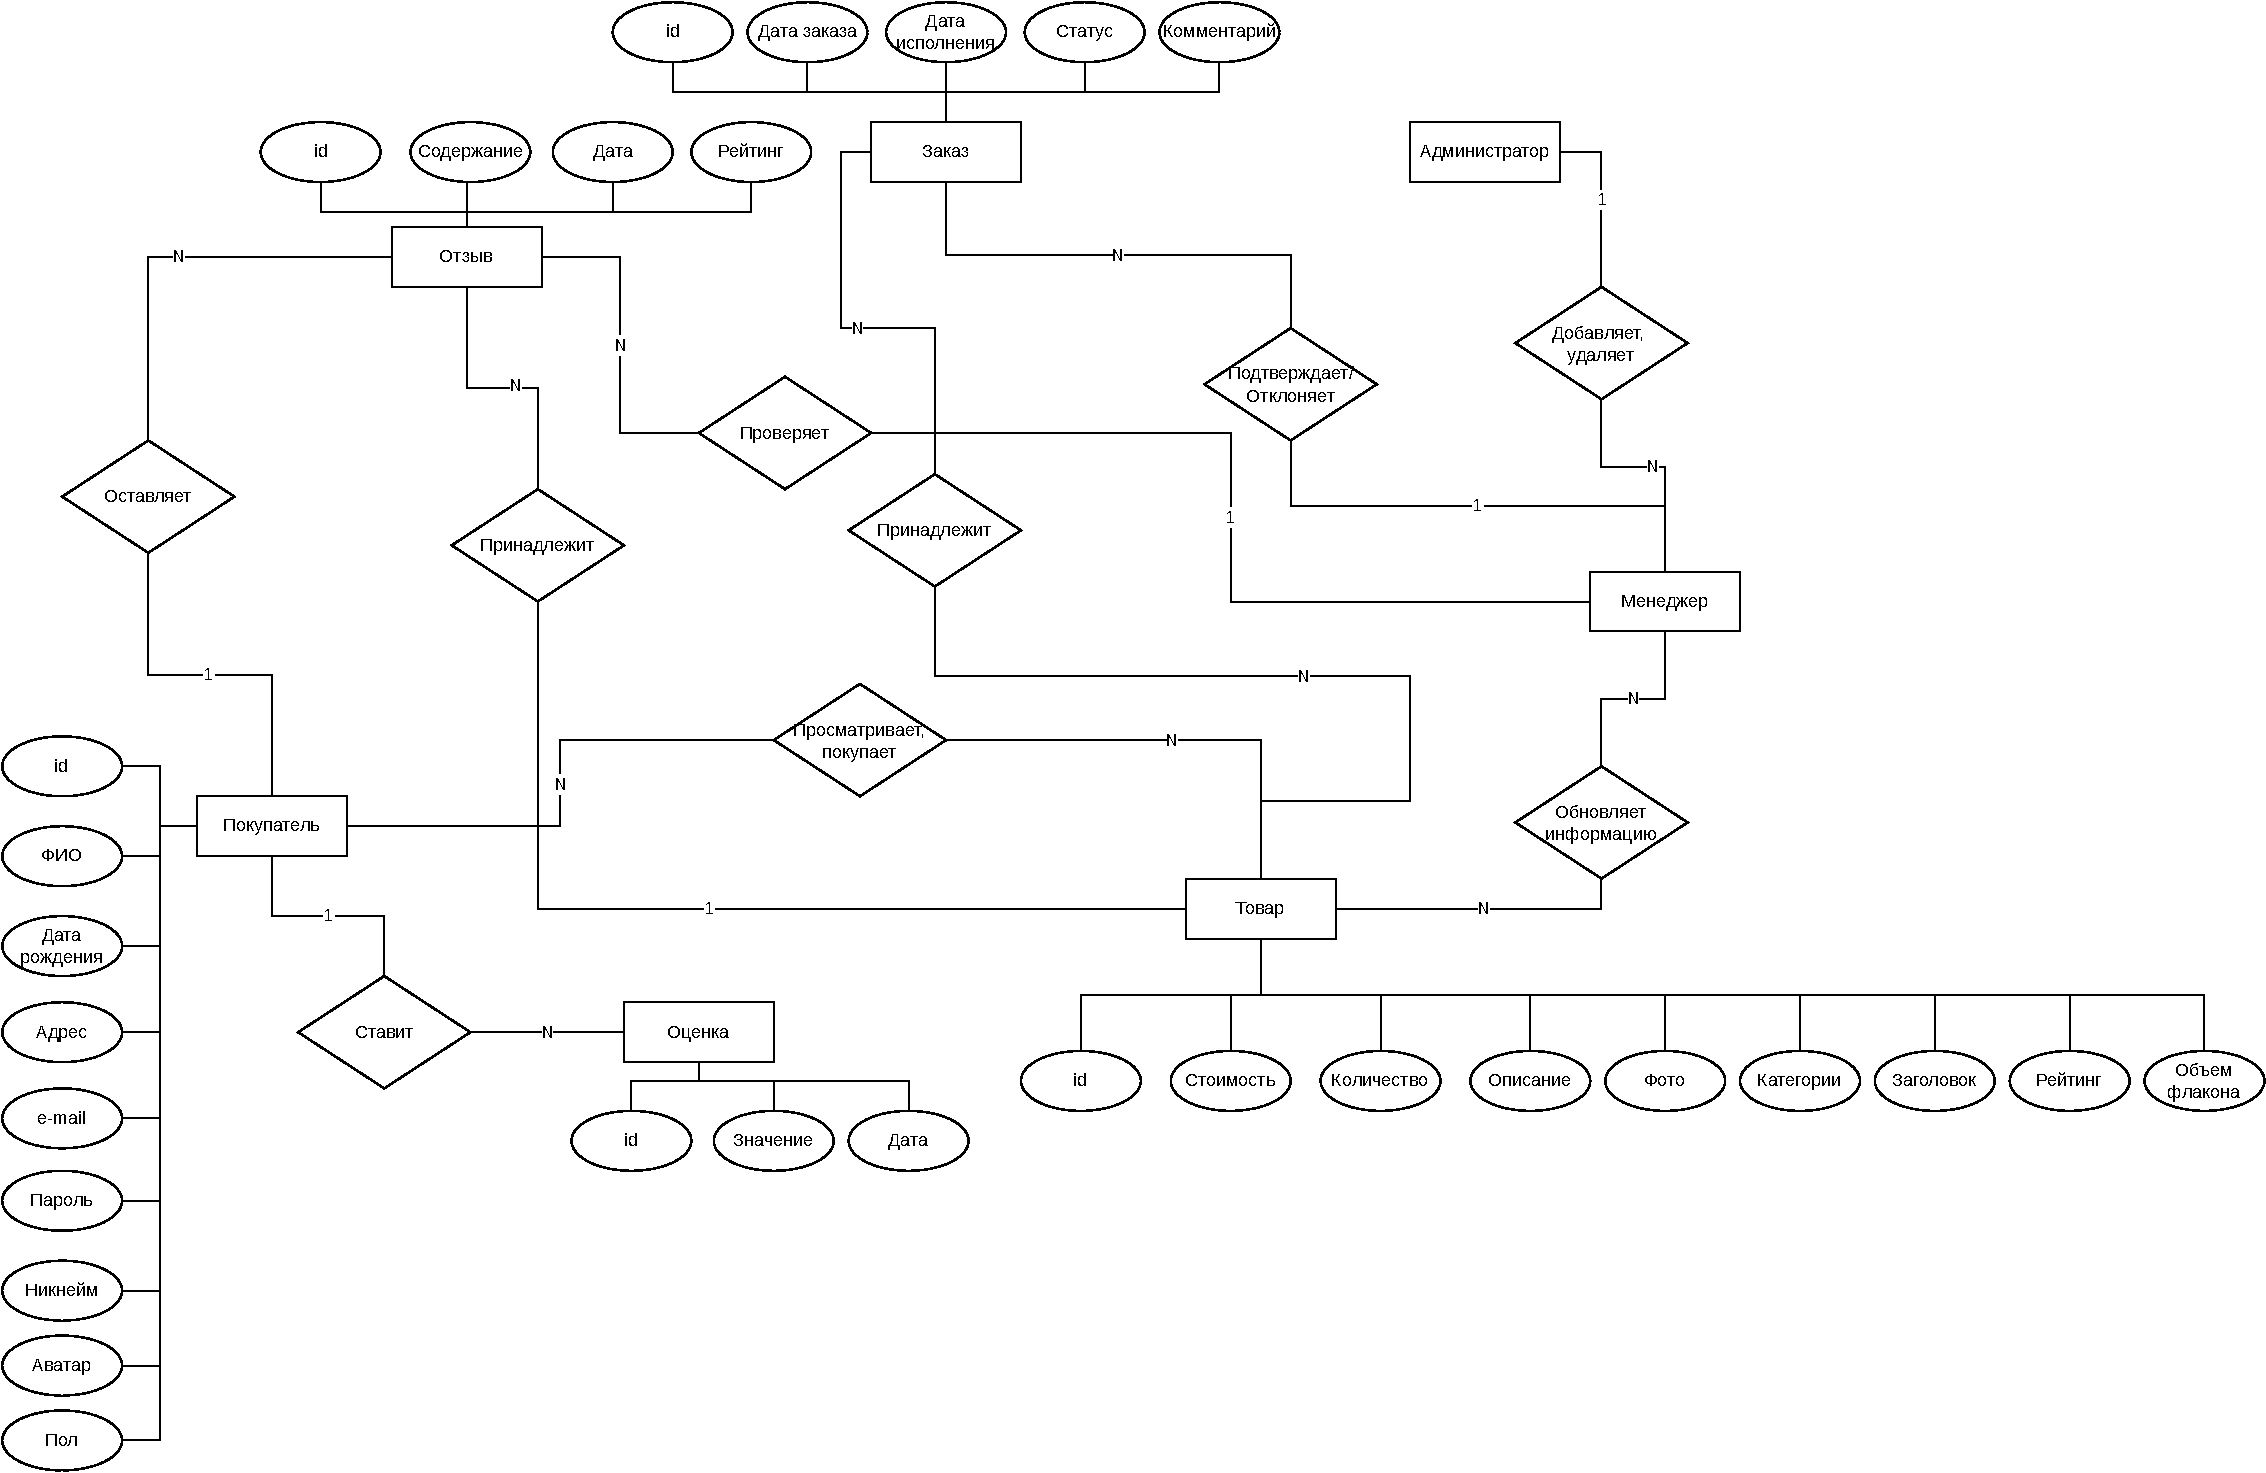
\includegraphics[scale=0.55, angle=90]{assets/er.pdf}
	\end{center}
	\caption{ER-диаграмма сущностей}
	\label{er_diagram}
\end{figure}

\section{Типы пользователей}

\captionsetup{singlelinecheck = false, justification=raggedright}
\begin{table}[h!]
	\begin{center}
		\caption{Типы пользователей и их функционал}
		\begin{tabular}{ |p{5cm}|p{11cm}| }
			\hline
			\textbf{Тип пользователя} & \textbf{Функционал}\\ \hline
			Покупатель & Просмотр каталога продукции и информации о товарах, написание отзывов и постановка оценок\\ \hline
			Менеджер & Просмотр каталога продукции и информации о товарах\newline Просмотр информации покупателей, просмотр информации о заказах, подтверждение и отклонение заказов, обновление продукции и информации о ней, модерация комментариев пользователей\\ \hline
			Администратор & Просмотр каталога продукции и информации о товарах\newline Просмотр информации покупателей, просмотр информации о заказах, подтверждение и отклонение заказов, обновление продукции и информации о ней, модерация комментариев пользователей\newline Добавление и удаление менеджеров\\ \hline
		\end{tabular}
		\label{user-table}
	\end{center}
\end{table}		


На рисунке \ref{use_case} представлена Use-Case-диаграмма.

\captionsetup{singlelinecheck = false, justification=centering}
\begin{figure}[h!]
	\begin{center}
		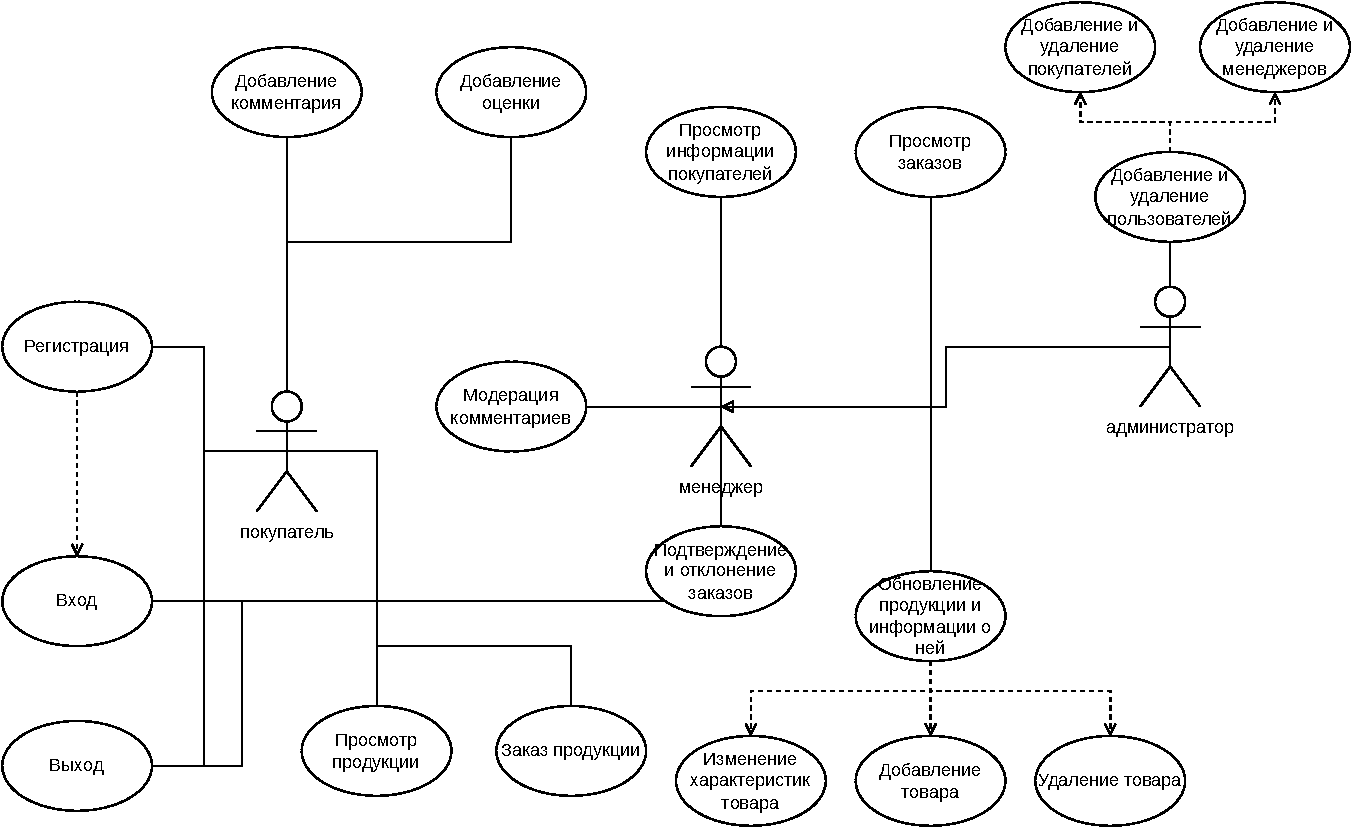
\includegraphics[scale=0.6]{assets/use_case.pdf}
	\end{center}
	\caption{Use-Case диаграмма}
	\label{use_case}
\end{figure}

\section{Описание существующих СУБД}
\textbf{Система управления базами данных} --- это комплекс языковых и программных средств, предназначенный для создания, ведения и совместного использования БД многими пользователями [1]. 

\subsection{Основные функции СУБД}
Основынми функциями СУБД являются:
\begin{itemize}
	\item управление данными во внешней памяти;
	\item управление данными в оперативной памяти с использованием дискового кэша;
	\item журнализация изменений, резервное копирование и восстановление базы данных после сбоев;
	\item поддержка языков БД.
\end{itemize}

\subsection{Классификация СУБД по модели данных}
\textbf{Модель данных} --- это абстрактное, самодостаточное, логическое определение объектов, операторов и прочих элементов, в совокупности составляющих абстрактную машину доступа к данным, с которой взаимодействует пользователь. Эти объекты позволяют моделировать структуру данных, а операторы --- поведение данных [2]. 

Существует 3 основных типа моделей организации данных:
\begin{itemize}
	\item иерархическая
	
Модель данных, в основе которой лежит иерархическая структура типа дерева. Дерево – это орграф, в каждую вершину которого кроме первой (корневой), входит только одна дуга, а из любой вершины (кроме конечных) может исходить произвольное число дуг. В иерархической структуре подчиненный элемент данных всегда связан только с одним исходным [3]. 
	\item сетевая
	
Основана на представлении информации в виде орграфа, в котором в каждую вершину может входить произвольное число дуг. Вершинам графа сопоставлены типы записей, дугам --- связи между ними [3].
	\item реляционная
	
В реляционной модели для отображения информации о предметной
области используется таблица, называемая отношением. Строка такой таблицы называется кортежем, столбец --- атрибутом. Каждый атрибут может принимать некоторое подмножество значений из определенной области --- домена.

Табличная организация БД позволяет реализовать ее важнейшее преимущество перед другими моделями данных, а именно возможность использования точных математических методов манипулирования данными,
и, прежде всего, аппарата реляционной алгебры и исчисления отношений.

К другим достоинствам реляционной модели можно отнести наглядность,
простоту изменения данных и организации разграничения доступа к ним [3]. 
\end{itemize}

\section*{Вывод}
\addcontentsline{toc}{section}{Вывод}

Поскольку реляционная модель базы данных является наиболее широко используемой и удобной, а также имеет возможность изменения базы данных без глобальных изменений программного обеспечения, то для реализации данного проекта была выброана именно она.

В данном разделе была произведена формализация поставленной задачи, описан необходимый функционал с распределением по ролям, проанализорованы модели базы данных и выбрана реляционная модель.